\section{Rendering pipeline}
\label{sec:opengl_rendering_pipeline}
Now that we know what a VBO is, we are ready to render the objects described by a set of VBOs on the screen. First we activate the data we want to render by telling the graphics card (of course by using the OpenGL API) which VBO identifier represents the positions, colors, normal vectors and texture coordinates. Then, we ask the GPU to render the activated data as the primitive the vertices represent (we know if the vertices should be rendered as triangles, quads or lines).\\
We can now make full use of the parallel architecture of the GPU. On a high end NVIDIA graphics card\footnote{Such as the NVIDIA GTX Titan. At the time of writing, it costs about 8000 NOK on \url{http://www.komplett.no}.}, there are often more than 2000 cores available to run small programs called \textit{shaders} that process the input data from vertices to the final image rendered on the screen. The shaders are written in a programming language called GLSL\footnote{GLSL (OpenGL Shading Language) is a programming language with syntax similar to C. It provides a set of linear algebra operations that are heavily used in computer graphics.} and are compiled on the GPU runtime. The full job of processing all the vertices calculating the final color values for all the pixels are distributed on these cores. In this section we discuss the different rendering steps in what's called the \textit{rendering pipeline} that are relevant to develop the visualization tools in this thesis. In figure \ref{fig:opengl_rendering_pipeline} we have illustrated the rendering pipeline containig the stages that we have used. 
\begin{figure}[h]
\begin{center}
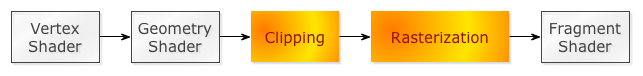
\includegraphics[width=\textwidth, trim=0cm 0cm 0cm 0cm, clip]{opengl/figures/pipeline.png}
\end{center}
\caption{Diagram of the OpenGL rendering pipeline. The gray boxes are shader steps (the shader programs can be written by the user). Each vertex is processed in the vertex shader before it is sent to the geometry shader that can create zero or more vertices based on the input vertex. Each vertex is then analyzed in the clipping program that removes vertices that cannot be rendered. The rasterization program creates a two dimensional image of every triangle so that the fragment shader can merge everything to color values per pixel on the screen. Not that the full pipeline contains more steps, but these are the relevant stages for understanding what our visualization tool does.}
\label{fig:opengl_rendering_pipeline}
\end{figure}
\subsection{Ins, outs and uniforms}
\label{sec:opengl_uniforms}
As we have already mentioned, the shaders are small programs run in parallel. Each shader gets some input data which are called \textit{input}-variables. These are specific values for this \textit{instance} of the shader, for example the position vertex for a particle. The shader then usually calculates \textit{something} (a common task in the first shader stage is to convert a vertex from the model space to the projection space), before it sends a variable to the next step in the pipeline. The variables going out of a shader is of course called an \textit{output}-variable. Just to be sure we understand; the next shader gets this \textit{output}-variable as an \textit{input}-variable for further processing.\\
But there are of course some variables that are constant through the whole rendering process. If all the particles have the same color, we don't need to specify the color per atom (this would use a lot of extra bandwidth on the GPU). Variables like this should be sent to the GPU as so-called \textit{uniform}-variables. They are available in all instances of every shader stage.
\subsection{Vertex shader}
The vertex shader is executed once per vertex in the input VBOs. It specifies which input vertex that is to be interpreted as the position, color, normal vector and/or texture coordinate if they are specified. The input position vertex is usually in the model space which are local coordinates for this specific object. A typical vertex shader applies the Model View Projection matrix on the vertex, transforming it from the model space to the projection space which often is assumed in the later pipeline stages. The latter may be done on the geometry shader instead if a three dimensional object is created at that stage.
\subsection{Geometry shader}
Each vertex from the vertex shader is a part of a primitive (such as \textit{GL\_POINTS} or \textit{GL\_TRIANGLES}). A geometry shader takes a primitive (i.e. a set of vertices, each processed by the vertex shader) as input and outputs zero or more primitives that may be of another type than the input primitive. A typical use is to describe a geometrical object (this could be a sphere or a tube) on the geometry shader so that the input primitive is just one single vertex; the position. This significantly reduces the memory and bandwidth usage on the GPU which usually gives great performance improvements.\\
The geometry shader can also be run in \textit{instancing mode} which means that the shader program is run a given number of time per vertex with an invocation id given. If a particle system obeys periodic boundary conditions, we can for example use the geometry shader instancing to add 26 periodic copies of the system making the system look larger than it is. 
\subsection{Clipping}
After the geometry shader has decided which primitives we want rendered, some of the vertices may not be visible on the screen. They can be behind the camera, too far to the right or in some way outside the camera view. When we in the final stages (the fragment shader) are going to decide colors on every pixels, we don't need to compute primitives that does not contribute to the final image. This is called clipping and is a very simple process to perform in the projection space. All vertices outside the clip volume (the volume that will be rendered) will be discarded and not computed at the rasterization stage.
\subsection{Rasterization}
The rasterization program will for each primitive determine which pixels that are a part of the primitive. Each active pixel will have interpolated colors and texture coordinates as described in subsection \ref{sec:opengl_texture_interpolation} before we reach the fragment shader, the final stage in the rendering pipeline.
\subsection{Fragment shader}
The fragment shader is executed one time \textit{per pixel} for each of the primitives that contributes to that pixel. 